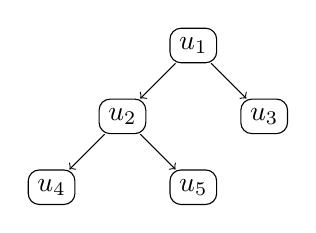
\begin{tikzpicture}[scale=0.9, 
				    state/.style={draw, rounded corners, fill=none,
				    			  text centered, text=black}]
	\node[state] (u1) at (7, 2) {$u_1$};
	\node[state] (u2) at (6, 1) {$u_2$};
	\node[state] (u3) at (8, 1) {$u_3$};
	\node[state] (u4) at (5, 0) {$u_4$};
	\node[state] (u5) at (7, 0) {$u_5$};
	\path[->] 	(u1)  edge   (u2);
	\path[->] 	(u1)  edge   (u3);
	\path[->] 	(u2)  edge   (u4);
	\path[->] 	(u2)  edge   (u5);
\end{tikzpicture}
